\label{Experiments}
\section{Experiments}


Some experiments were conducted to verify the correctness of the algorithm and its running time. The results were computed for both algorithms: Misra-Gries and our algorithm.
The experiments were run on the same machine. Environment specification:

\begin{description}
  \item[Processor] Intel Core i7-2760QM 2.20 GHz
  \item[Memory] 8GB, 1,333MHz DDR3
  \item[Hard drive] 1TB, 5,400rpm
\end{description}

\begin{table}[ht]
\caption{Results for Misra-Gries algorithm}
\centering
\begin{tabular}{c c c c c}
\hline\hline
\begin{tabular}{@{}c@{}}IMDB \\ Input Size\end{tabular}&
\begin{tabular}{@{}c@{}}Roles \\ Number\end{tabular}&
\begin{tabular}{@{}c@{}}Running \\ Time (h)\end{tabular}&
\begin{tabular}{@{}c@{}}Result \\ Triplet\end{tabular}\\ [0.5ex]
\hline
100\%&48 967 421&38.6&\{760909, 406612, 80307\} \\
\hline
\end{tabular}
\label{resMisraGries}
\end{table}

As predicted in section \ref{AnalysisMisraGries}, the running time of Misra-Gries in our setup was expected to be long. The results in table \ref{resMisraGries} support this. The long running time comes from the fact that there are movies with a large number of actors. For these, the algorithm computes all possible triplets combinations. Furthermore, the bigger the cache, the longer the running times. The above experiments were performed with a chache size 20 000 triplets. More about the chache size in section \ref{MisraGries}

\begin{table}[ht]
\caption{Results for our algorithm}
\centering
\begin{tabular}{c c c c c c}
\hline\hline
\begin{tabular}{@{}c@{}}IMDB \\ Input Size\end{tabular}&
\begin{tabular}{@{}c@{}}Roles \\ Number\end{tabular}&
\begin{tabular}{@{}c@{}}Building \\ Time (sec)\end{tabular}&
\begin{tabular}{@{}c@{}}Running \\ Time (sec)\end{tabular}&
\begin{tabular}{@{}c@{}}Result \\ Triplet\end{tabular}&
\begin{tabular}{@{}c@{}}Result \\ Movies\end{tabular}\\ [0.5ex]
\hline
100\%&48 967 421&393.409&8.282&\{150878, 215408, 215564\}&130\\
50\% (seg-0\_2)& 24 434 967 & 200.750 & 4.795    & \{150878, 215408, 215564\} & 130 \\
50\% (seg-1\_2)  & 24 532 454 & 196.157 & 3.356    & \{157955, 651761, 329494\} & 101 \\
25\% (seg-0\_4)  & 12 339 915 & 98.711  & 2.142    & \{33500, 316918, 761020\}  & 84  \\
25\% (seg-1\_4)  & 12 273 033 & 98.430  & 2.095& \{41669, 341023, 338852\}  & 94  \\
25\% (seg-2\_4)  & 12 101 052 & 95.708  & 2.150& \{150878, 215408, 215564\} & 130 \\
25\% (seg-3\_4)  & 12 259 421 & 97.868  & 2.061 & \{157955, 651761, 329494\} & 101 \\
10\% (seg-0\_10) & 4 899 811  & 39.729  & 1.225 & \{33500, 316918, 761020\}  & 84  \\
1\% (seg-0\_100) & 489 009    & 4.242   & 0.183  & \{33500, 316918, 761020\}  & 84  \\
\hline
\end{tabular}
\label{results}
\end{table}

\begin{figure}[ht!]
\centering
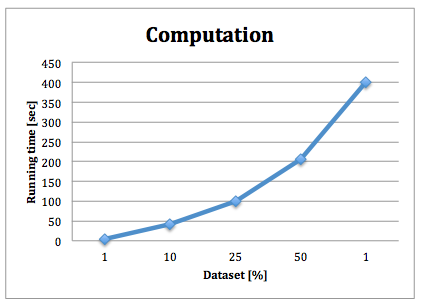
\includegraphics[width=100mm]{resources/graph.png}
\caption{Algorithm Running Times}
\label{ourAlgorithmRunningTimes}
\end{figure}


The analysis made in section \ref{OurAlgorithmAnalysis} predicted, the worts case running time is O(\(n^3\)). As can be seen in table \ref{results}, the running times are obviously within the bounds. Meaning that doubling the problem size increases the computational time with a factor of less than 3.

\subsection{Parallelisation}
\label{ExperimentsParallelism}
As already mentioned, the graph is built in such a way, that the data is easy to split. This property allows for easy parallelisation. Parallelisation can be achieved by simply dividing the data into groups and processing them parallel.
We ran our experiments on an 8-core machine, which allows for a maximum of 8 threads running simultaneously. This makes the algorithm almost 8 times faster. Table \ref{resParallelExecution} show the time needed to process 100\% of the data set with single thread and eight threads running concurrently.
\\
Important to note here, is what happens in the case of when the data set does not fit in memory. We could have multiple parallel executions in this case. Each parallel execution will be performed sequentially. Take for example the case when the whole data set is of size 10GB, while we have 4GB available. We can have 3 sequential executions (2x4 + 1x2). Each of them will use all the available cores - will be executed in parallel.


\begin{table}[ht]
\caption{Results for Parallel Execution}
\centering
\begin{tabular}{c c}
\hline\hline
\begin{tabular}{@{}c@{}}Thread \\ Count\end{tabular}&
\begin{tabular}{@{}c@{}}Running \\ Time (sec)\end{tabular}\\ [0.5ex]
\hline
1&401.691\\
8&53.487\\
\hline
\end{tabular}
\label{resParallelExecution}
\end{table}
